
%----------------------------------------------------------------
% Concept
%----------------------------------------------------------------
\section{Privacy Intrusion through AR and CV Technologies}

To demonstrate the risk of privacy intrusion of emerging augmented reality and computer vision technologies, we identified three factors that we believe to enable malicious users to abuse these technologies.

% -(factor 1) Advancement of augmented reality technologies (robustness, accuracy) and ease of integration (AR libraries) will presumably lead to a surge in mobile applications utilizing such features. \\
% -Current AR applications are often developed for entertainment purposes or as feature showcase, but with increasing maturity of the technology, conceivable use cases appear in a wide range of domains, e.g. information display in professional environments, medical application, support of sensory functions, etc. \\
First, advancements of augmented reality technologies, in particular in terms of robustness and accuracy, may lead in the future, and in parts already have led, to a surge in mobile applications utilizing such features.~\cite{HCI-049}
Their ease of integration is greatly enhanced by dedicated libraries offered by operating system vendors, such as Google and Apple.\\
Increasing computational power in consumer devices allows these libraries to use 2D images to compute the depth of the room, instead of having to rely on dedicated hardware to read the depth.
While currently AR applications are often developed for entertainment purposes or as a feature showcase, one can expect AR technology to become common in more diverse areas, such as information display in professional environments, medical applications, or support of sensory functions.\\
% - (factor 3) By necessity, AR applications are granted permission to access the camera input of the mobile device. This opens up a visual window into the immediate and intimate vicinity of the user, often in their homes or work places. \\
Secondly, this poses a danger, as AR applications are granted permission to access the camera input of the mobile device by necessity.
With AR applications being used in diverse areas, as outlined in point two, highly sensitive information will be made visible to the mobile device and opens up a visual window into the immediate and intimate vicinity of the user, often in their homes or workplaces.\\
% - Additionally, advancements in computer vision increase the computational interpretability of pictures or even extensive near real time analysis of video feeds.
Third, progress in the area of computer vision increases the computational ability to interpret pictures in machine-readable formats. This goes to the extent that even the real-time or near real-time analysis of video feeds becomes possible. Otherwise, emerging offers in cloud infrastructure by, for example, Google offer services specifically designed to quickly and efficiently process image input at scale.~\cite{VisionAPI}

% -> \textbf{large-scale data mining of the user's analog environment becomes  conceivable.}
Combined, advancing computer vision allows large-scale data mining, while augmented reality places the camera sensors right in the user's most sensible environment.
Additionally, AR games may even allow manipulating the user into navigating to specific areas that the malicious application considers particularly interesting, by moving important game play elements in those areas and prompting the user in this way to point the camera at specific points of interest.

% - Malicious actor: Could uncover sensitive information that is heavily protected in the digital world.
As a consequence, a malicious actor aiming to steal data from users could uncover sensitive information that may be heavily protected from access in the public world but could be immediately revealed by legitimate actors with access to the area, if they use a compromised AR application.
% Possible desirable information could be tax identification numbers, bank account numbers, social security numbers, etc., i.e. anything that can often be found in plain sight on sensitive documents but is well-encrypted in digital representations.
Important information that could be accessed in the setting of a regular consumer game includes all information that is printed out and would otherwise be well protected in a digital setting, such as tax identification numbers, bank account numbers, or social security numbers.

% -Authoritarian governments: Surveillance use cases; automatic detection of contraband or illicit material, even cues for dissident tendencies. Potential for integration of analysis capabilities on the OS level with e.g. a custom Android distribution.
Authoritarian governments, however, may receive free and voluntary access to a huge number of surveillance cameras all over the country if an application is modified accordingly. This may allow automatic detection of contraband or illicit material, or even cues for dissident tendencies. Large-scale actors like a government may even have the potential for integration of analysis capabilities on the operating system level, by using for example a custom Android distribution.
This would evidently allow them to have the camera record at all times, independent of an application, but via AR they also receive the option to navigate the user and incentivize moving the phone's camera around the room.

% - profit-driven actor: Allows the creation of precise consumer profiles for targeted advertising and audience selection. Could provide insights that classical profiles generated by online behaviour analysis lack.
Further, profit-driven actors could use the gathered information to gain insights into the user's non-digital life, to create even more precise consumer profiles for targeted advertising and audience selection.

% However, mere panning over a room's interior does not provide images with a high enough resolution to gather most often fine-printed information.
Many of these use cases currently require images of very good quality.
Techniques like optical character recognition (OCR), for example, which enable the automatic processing of captured text, require close-up shots and sufficient picture clarity.
With the Demon Go prototype, we demonstrate an approach where the user is led into providing these necessary close-up shots.
To hide this exploitation from the user, we align the requirements on the camera feed with plausible and engaging game mechanics.
We specifically designed the prototype in a way that the exploitation aspect remains as well hidden as possible, and appears to merely be using features required for the game to work.

\section{Game Concept}
\label{sec:concept}

In order to provide a proof of concept that the combination of AR and computer vision technologies may be used in a malicious way, we created the application \emph{Demon GO}.
As the name implies, the game concept is heavily inspired by the already mentioned globally successful AR game Pokémon GO and the book series Bartimaeus. The book revolves around a world in which demons and other magical creatures exist, only visible to other demons or humans who use special devices.~\cite{stroud2004bartimaeus}

\subsection{Data Collection Requirements}
\label{subsec:collectingdata}

For the success of the data collection, it is crucial that we are able to direct the attention of the users and therefore also their camera in the direction of interesting points within their vicinity.\\
The best way to achieve this is to divide the AR part of the game into two different sections.
In the first section, which is called the \emph{scanning phase}, as much as possible of the surroundings of the player should be scanned and roughly analyzed to identify points of interest.
In the following \emph{capturing phase} the player should be forced to take a closer look at identified points of interests and thus provide higher resolution camera frames of the desired locations.
Those can later be used for more precise analysis, such as the application of OCR algorithms.\\
Additionally, the geolocation of the users can be gathered if gameplay elements are bound to the interaction at real-world locations.

% Welche Daten sammeln wir dabei? → “Dämon als Datenpunkt”
%- capturing a demon: two phases
%- phase 1: scanning, demon is flying around randomly while the captured camera frames are processed
%- camera frames are rated by specific metrics. goal is to identify interesting points (e.g. text, brands, faces) to send the user to -> best frames are PoI
%- phase 2: capturing, demon flies to PoI to force the user to point camera at it and "cast the spell" (i.e. hold phone relatively even while pointing at the PoI and with half of the view covered by pattern/finger)
%- more detailed processing of captured frames
%(- also geolocation of user can be captured when he places stashes/moves around to attack others)

% Berechtigungen ergeben Sinn
Furthermore, it is indispensable that players do not become suspicious and regard the app as a potential threat to their privacy.
Therefore, every permission which has to be granted is reflected in the game and each permission's necessity for a functioning game should be obvious to players:
\begin{itemize}
    \item The camera access is needed to ensure that ARCore is working and is able to display demons in the real world.
    %\item The geolocation of the users is needed to track their position in the real world and ensure that they are only able to place, rob (and conceptually attack and defend) stashes which are close to them.
    \item The geolocation of the users is needed to track their position in the real world and ensure that they are only able to interact with position-based gameplay elements if they are close enough in the real world. 
    %\item Internet access is also required because the information about the stashes, players, and demons need to be synchronized between different players.
    \item Internet access is also required because the information about other players and certain locations need to be synchronized between different players.
\end{itemize}

When it comes to data volume usage, it is important to keep the used resources as low as possible. 
Thus, it is not feasible to stream all the captured frames directly to the server, since frames captured with a resolution of 1080 by 1920 pixels will usually be larger than a couple hundred kilobytes, if not multiple megabytes, depending on the compression.
Especially when players are connected to the Internet through a connection that they pay for, they will get suspicious if the game will use a major part of their data allowance.
In any case, it would be unusual that an app would need as much bandwidth while claiming to merely synchronize necessary game information between players.\\
Even if we could assume that all players have enough data allowance to constantly stream all the data, there would be two limitations left:
First, bandwidth may not be available all the time when users try to catch demons, which could be a problem in regions where no fast mobile Internet is available.
Second, the server may not be able to process all the uploaded frames because some of the employed algorithms take a couple of seconds to process a single frame.
Especially if we want to analyze the camera feeds of a large number of users, this becomes unfeasible.\\
To solve all these issues, we preprocess and preselect frames based on a scoring mechanism on the user's phone which will guarantee that only the best frames in terms of quality and interest will be sent to the server.


\subsection{The Player's Objective}

The game's main goal is to control as much territory of the augmented world as possible.
Players need to place public stashes at locations in the real world which mark their reign and have a specific range of influence (\autoref{fig:map}). 
To defend those stashes against attackers the player needs to collect demons which are flying around in the augmented reality world, waiting to be captured by the players. 

\begin{figure}
    \centering
    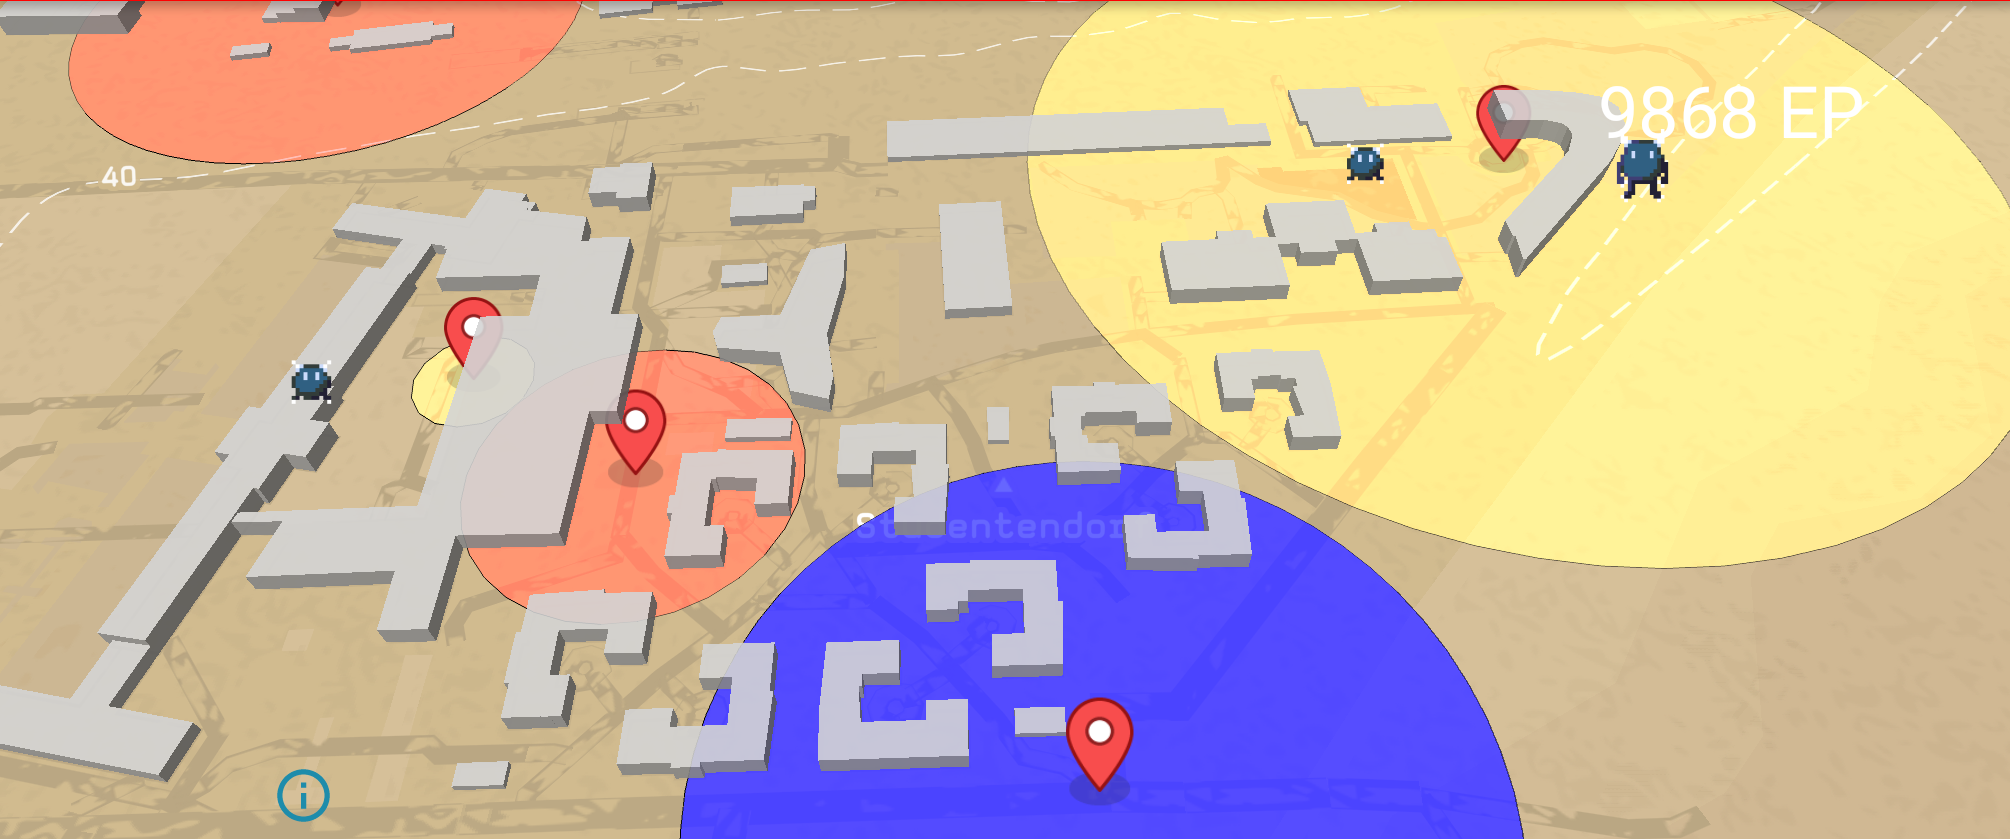
\includegraphics[width=8cm]{graphics/map.png}
    \caption{Screenshot of the map with stashes, their areas of influence, and their defending demons}
    \label{fig:map}
\end{figure}


Moreover, players gather energy points (EP) in the game by releasing their previously caught weaker demons. They can then use the EP to summon stronger demons for a more effective defense.

Besides defending stashes, demons can also be used to attack stashes of other players and have a direct influence on the radius and the maximum EP capacity of the stashes on which they are placed.

As players can only hold a certain maximum capacity of EP in their \enquote{in-game purse}, they need to place them in stashes where the EP can theoretically be stolen by opponents. 
Hence, the players are motivated to defend their stashes with stronger demons which indirectly forces them to first catch more demons in the augmented world to gain more EP.

%- 4 elements: gathering energy points (the in-game currency), capturing demons, beat their demons protecting the stashes

%- (for implementation: the stronger the demons, the bigger the range of influence --> direct correlation) 
%- stashes can only be placed at current location

%- in the area of influence of one player it's not possible for other players to place their stashes --> hence players are forced to attack hostile stashes to decrease their area of influence (by killing defending demons) or ideally to destroy the whole stash and steal in-game currency called energy/experience points placed by the defender

\subsection{Getting Demons}
\label{subsec:demons}

\begin{figure}[t]
\centering
  \subcaptionbox{Sphere flying through room, player is trying to shoot it
  \label{fig:sphere}}{%
    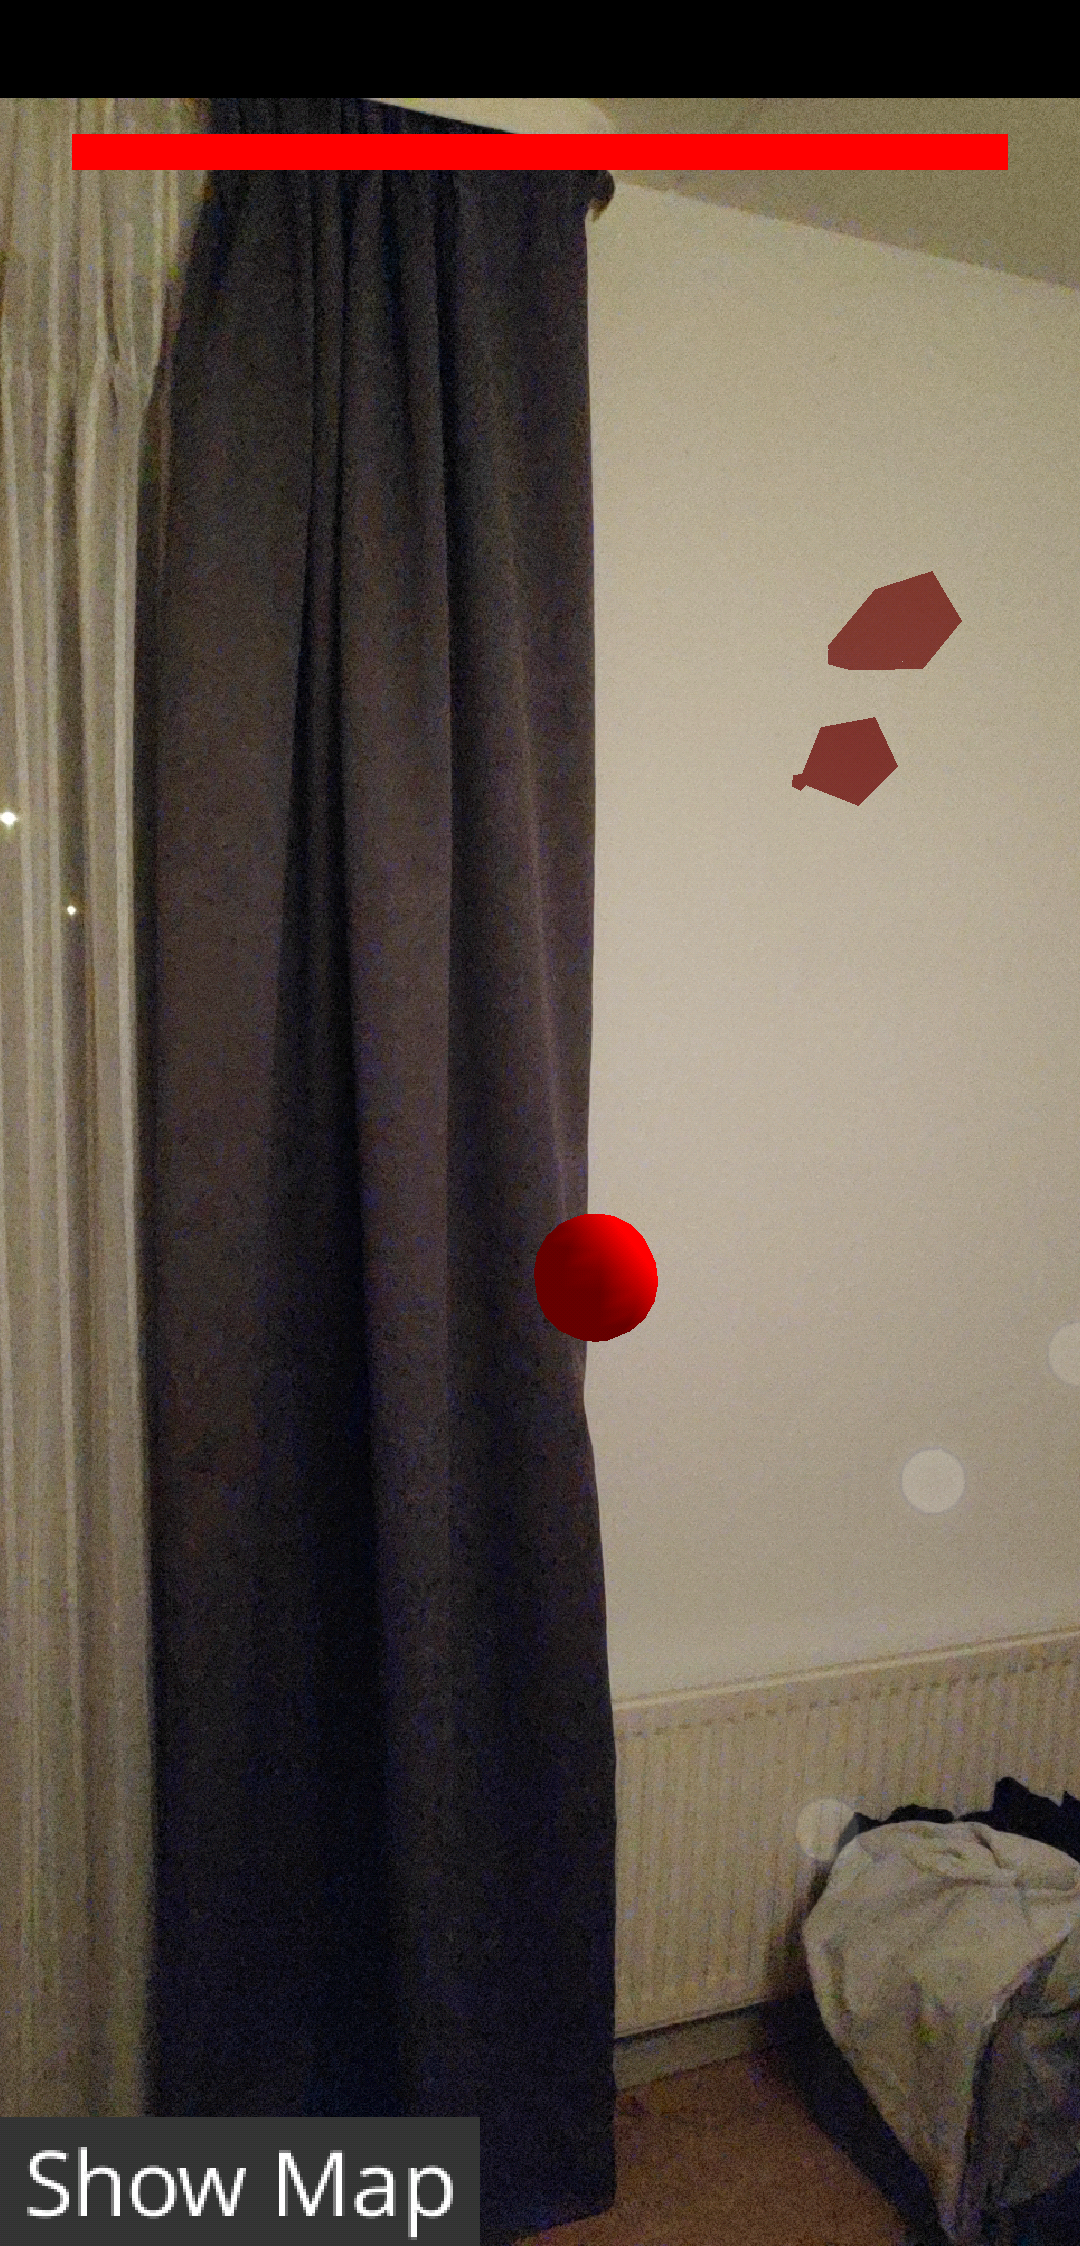
\includegraphics[width=4cm]{graphics/sphere.png}}\quad
  \subcaptionbox{Demon is unleashed, player is close enough to cast spell \label{fig:demon}}{%
    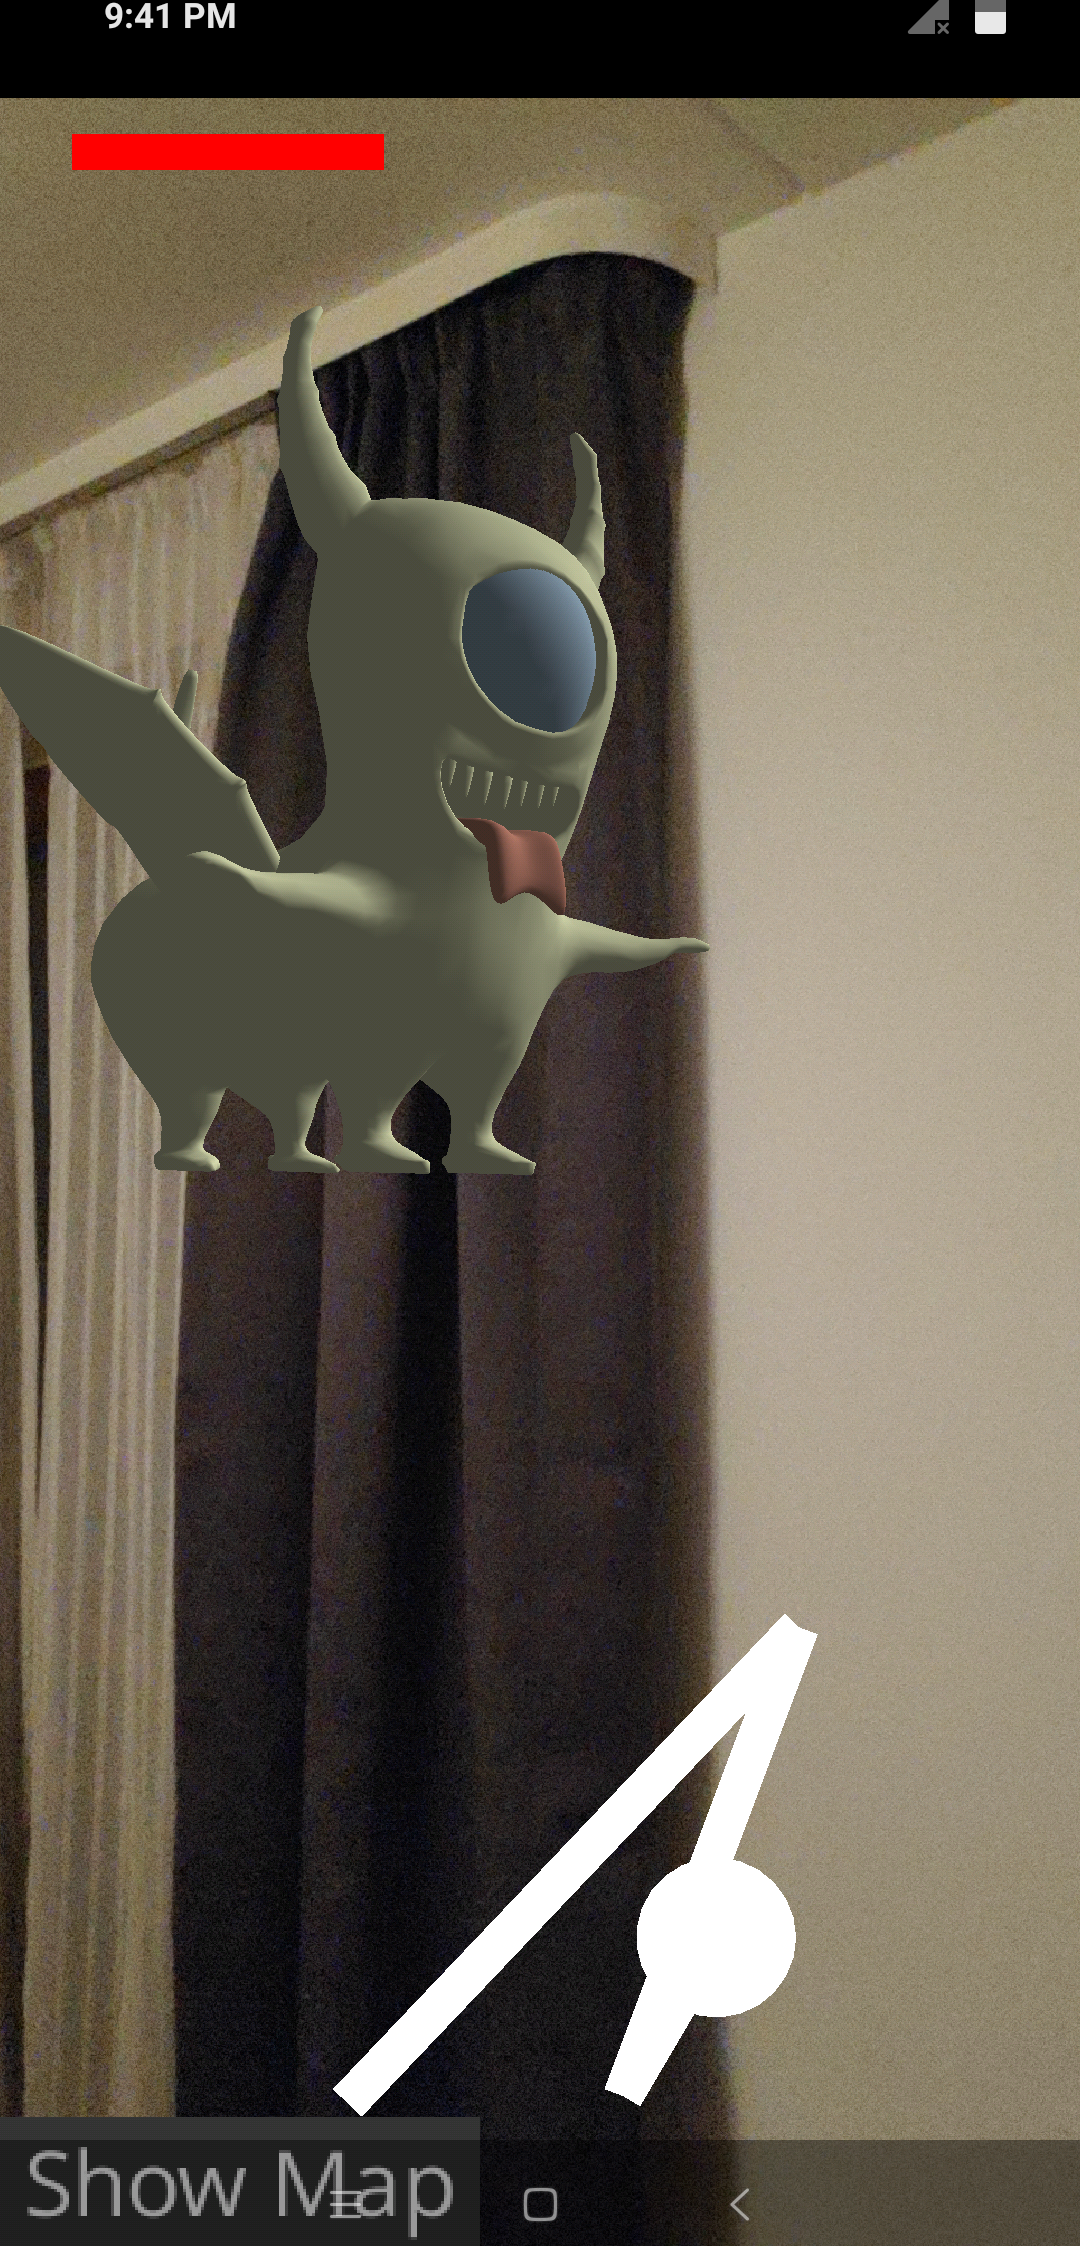
\includegraphics[width=4cm]{graphics/demon.png}}\quad
\end{figure}


To defend and attack stashes the player needs to collect demons.
The first of two possible ways is to find, follow, and fight demons that are present in the augmented reality world and can be seen through their \enquote{magic lense}, which corresponds to the augmented reality view in the Demon GO app.

To find a demon, players first have to search for flying spheres that represent demons in their hidden form as depicted in \autoref{fig:sphere}.
The sphere flies around quickly and changes its direction frequently, which gets players to scan as much of their surrounding area and thus allowing the system to both get an idea of the room and scan for potential points of interest.
To force the demon to appear properly, players need to tap (shoot) the sphere multiple times on their phone screen. This part of the gameplay is the previously mentioned \emph{scanning phase}.

The \emph{capturing phase} begins immediately after the demon emerged from its sphere (\autoref{fig:demon}).
It is now navigating towards points of interests that were derived from the camera stream in the \emph{scanning phase}.
To capture the demon, players first need to get close enough to it, which enables them to weaken it by \enquote{casting spells} in form of drawing specific patterns on the screen. 
By getting closer to the demon the player ideally provides the camera with a better view and angle onto the previously detected points of interest, which results in higher quality frames of potentially sensitive data for better data analysis. 
At the same time, the virtual demon hides the point of interest underneath it to not arouse any suspicion in the players, given that they are fully focused on drawing the pattern. To further ensure that the point of interest is covered, a smoke particle system is attached to the demon.

After multiple successful spell castings, which correspond to the player having visited all detected points of interest, the demon is captured and will be added to the player's demon collection. 
From there, it can be used to attack other stashes, defend own stashes, or be sacrificed in order to receive more EP.

The other intended, but not yet implemented way, to collect demons is to summon them.
To do so, the players need to be within reach of one of their stashes and pay a certain amount of EP to start the incantation.
Furthermore, the likelihood of a successful incantation depends on the reach of the stash, the strength of the defending demons and the strength of the demon that is being summoned.
This makes it very likely that players place a well-defended stash somewhere where they often stay or go, for example, their home, workplace, school, university, etc.
Hence, the user may disclose more private information, rather than providing more imagery of publicly accessible places.

\subsection{Stashes and EP}
\label{subsec:stashesandep}

%- mark territory of player (circle around stash)
As players have a maximum capacity of EP they can carry and strong demons can be expensive they need to store EP in stashes.
Those can only be placed at the current location of the user and their reach is visualized by a colored circle on the map, see \autoref{fig:map} for examples.
A player can have an unlimited amount of stashes, all of them being visible to all other players. 
%- have to be defended against attackers
%- range of influence can be extended by placing demons on them which furthermore defend the stashes against attackers 
%- also the max capacity of EP that the stash can hold increases with the strength of the defending demons

While in the reach of one stash, it is not possible to place other stashes - hence, players are forced to attack hostile stashes to decrease their area of influence, by defeating the defending demons, or destroying the whole stash to also steal the stored EP.
As players can currently instantly attack other stashes anywhere in the world we decided that EP from defeated stashes can only be picked up by players close to the stash.
That enforces players to regularly check if they are close to a defeated stash on the map to pick up the exposed EP, even though they did not destroy the stash.
%- forces players to place stashes in the real world 
%- provokes other players to limit their possible range of influence and steal the stashed EPs
%Furthermore, as stashes indirectly represent the players' game progress, we decided that they should be hard to destroy.

Stashes can have three different states which have different attributes and are depicted in \autoref{fig:map}.

\begin{itemize}
    \item A newly created stash with no EP in it is only visible to its creator as long as no demons defend it and no EP are stored in it.
    \item When a player deposited EP in a stash but did not place demons to defend or after every defending demon is defeated the stash is visible to everyone with a blue perimeter, showing that EP are free to collect for everyone in a specific range (currently 100 m).
    \item A stash that is currently defended by demons is either surrounded by a red perimeter for hostile stashes or a yellow perimeter for own stashes. 
Furthermore the perimeter range depends on the strength of the defending demons, currently implemented as a correlation to the sum of all maximal health points (HP) of the defending demons.
\end{itemize}

As players cannot see the defending demons of hostile stashes it is harder to predict how good stashes are defended.
A big perimeter also does not necessarily imply that the defending demons still have many HP due to the correlation of the radius to the maximal HP of the defenders and not to their current HP.
Besides that attackers also cannot see how many EP their opponents placed within a stash.
That allows bluffs in which players place many demons on a stash without storing EP in it to restrict the max area of other players' stashes.

%- stashes are visible to other players (on the map) and can be attacked by them (currently only one demon at the time) 

%\subsection{Attacking and Defending Stashes}
%\label{subsec:attackingstashes}

Battling stashes currently involves exactly two parties, an attacking demon and a static collection of defending demons which were placed on the attacked stash in advance.

%When the attacker wins the fight the EP of the defeated stash get exposed. 
%- is shown to everyone and everyone nearby can collect the EP by clicking on the stash (if he has enough capacity) --> currently user needs to be in a radius of 100 m around the stash 

%--> motivates players to move irl and to expose more documents/sensitive content

%- also motivates other players to check regularly if they have a defeated stash nearby to collect the EP

%[picture of defeated stash]

The fights are conceptualized that it's hard to destroy a stash as stashes and the deposited EP within them are basically the user's game progress and as one stash can theoretically be attacked by everyone at anytime.
Moreover opponent players obviously have the chance to ally up to pursue their common goal of decreasing a strong defender's range of influence.

%- very important to balance the summoning cost of different kinds of demons with the possible amount of EP an attacker can receive when destroying a stash


\subsection{Future Gameplay Ideas}
\label{subsec:futuregameplayideas}

Additional to the current implementation of the game we want to mention further ideas that could be implemented with more time and resources to get access to even more data and to further enhance the gameplay.

\begin{itemize}
    \item One additional feature we started implementing were Player-vs-Player (PvP) fights to get users to expose even more camera data.
    Besides our current data analysis PvP fights would also allow us to recognize and analyze facial images by guiding demons into the direction of the opponent player.
    \item To summon demons our main idea was to make the player draw and scan a specific symbol in the real world.
    Our assumption is that the players would probably draw that on a sheet of paper on top of their desk, possibly close to other documents that could be recognized by the data exploitation subsystem.
    \item An approach to make the game more interactive would be to enable allies and to e.g. allow trading EP, use shared stashes, summon demons in shared territory or defend stashes of other players.
    This would make the game more collaborative and could lead to a snowball-effect in which the game's popularity would benefit from many players recommending it to their friends.
    \item By calculating the time a demon needs to get to a stash dependant on the distance to it we could make the game more realistic and strategic. 
    Also showing attacking demons on the map could increase the addictive potential of the game as users could come up with different strategies for defending and attacking stashes, depending on the amount of incoming attacks and their times of arrival.
    %(as e.g. in other online multiplayer strategy games like Tribal Wars).
\end{itemize}



%- show the attacking demon on map next to the defenders and display current fight status over their icons


